\tabulinesep=4pt

\begin{frame}{Motivation}
  Die meisten Geräte basieren auf Unix
  \begin{itemize}
    \item Server, Cluster, Supercomputer
    \item Smartphones
    \item Router, Drucker, …
  \end{itemize}
  Wissenschaftliche Programme werden in der Regel für Unix geschrieben
  \begin{itemize}
    \item Bedienung über Kommandozeile
    \item Wichtige Programme haben keine GUIs
    \item z.\,B. bei der Bachelor- oder Masterarbeit
  \end{itemize}
\end{frame}

\begin{frame}{Motivation}
  \begin{itemize}
    \item Kommandozeile ist in vielerlei Hinsicht überlegenes Bedienkonzept
      \begin{itemize}
        \item Die meiste Zeit beim wissenschaftlichen Arbeiten verbringen wir in der Kommandozeile (auch CLI, Command Line Interface)
      \end{itemize}
    \item GUIs (Graphical User Interface) verstecken die Details
    \item GUIs sind nicht böse oder schlecht, man muss nur wissen, was dahinter steckt
    \item In der Kommandozeile ist alles automatisierbar
      \begin{itemize}
        \item Wenn man etwas zum dritten Mal tut, sollte man ein Skript dafür schreiben
      \end{itemize}
    \item Arbeiten in GUIs ist nur schwierig reproduzierbar
  \end{itemize}
\end{frame}

\begin{frame}{Terminal-Emulatoren}
  \begin{columns}
    \begin{column}{0.5\textwidth}
      \begin{itemize}
        \item Terminals sind im ursprünglichen Sinne Hardware und wurden durch den Personal Computer ersetzt
        \item Terminal-Emulatoren oder auch Terminalprogramme sind Programme die Terminals auf einem PC emulieren
        \item Beispiele für graphische Terminal-Emulatoren sind:
        \begin{columns}[t, onlytextwidth]
          \begin{column}{0.1\textwidth}
          \end{column}
          \begin{column}{0.3\textwidth}
          \textbf{Linux}
          \begin{itemize}
              \item xterm
              \item GNOME Terminal
              \item kitty
              \item tilix
          \end{itemize}
          \end{column}
          \hfill
          \begin{column}{0.3\textwidth}
          \textbf{Windows}
          \begin{itemize}
              \item Windows Konsole
              \item Windows Terminal
          \end{itemize}
          \end{column}
          \hfill
          \begin{column}{0.3\textwidth}
          \textbf{macOS}
          \begin{itemize}
              \item iTerm2
              \item Terminal
          \end{itemize}
          \end{column}
          \end{columns}
      \end{itemize}
    \end{column}
    \begin{column}{0.5\textwidth}
      \begin{figure}
        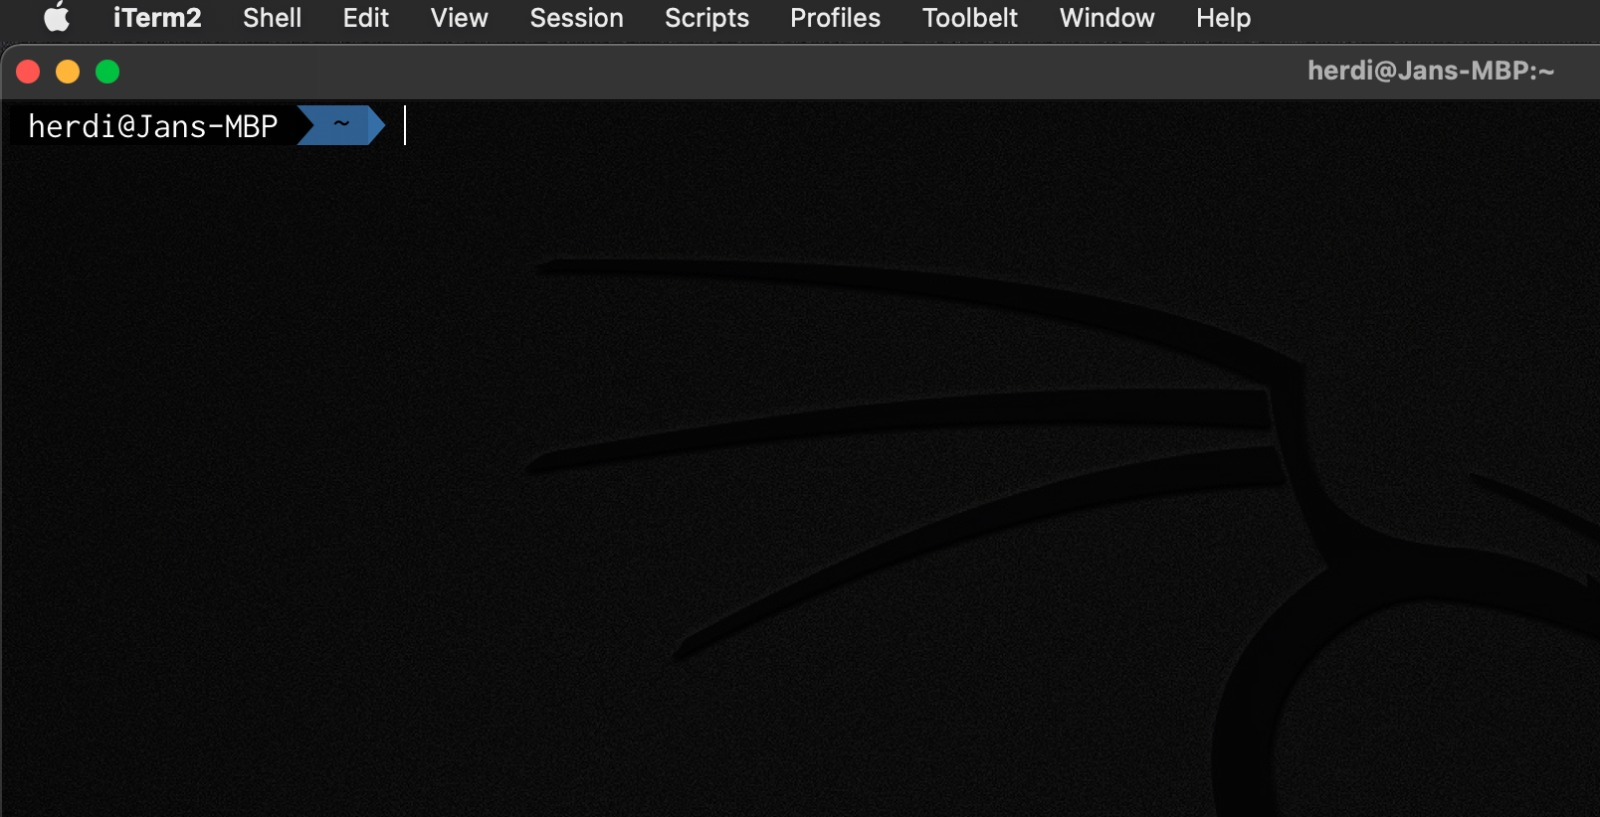
\includegraphics[width=0.7\textwidth]{images/iterm2.jpg}
      \caption*{iTerm2 in macOS}
      \end{figure}
      \begin{figure}
        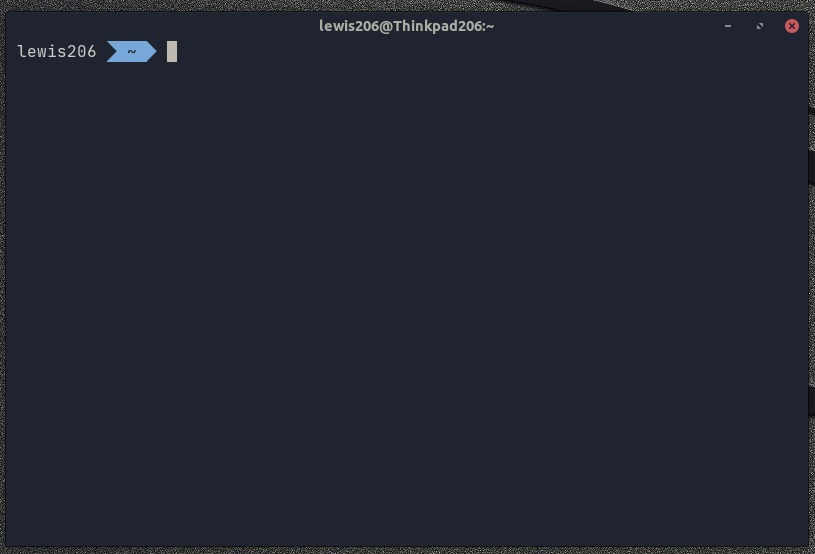
\includegraphics[width=0.7\textwidth]{images/gnome-terminal.jpg}
      \caption*{GNOME Terminal in Linux}
      \end{figure}
    \end{column}
  \end{columns}
  
\end{frame}

\begin{frame}{Tastaturkürzel}
  Es gibt verschiedene Tastenkürzel, die sich je nach Terminal-Emulator unterscheiden
  \vspace{1em}\\ 
  \begin{tabu}{>{\ttfamily}l | >{\ttfamily}l | >{\ttfamily}l | X[,L]}
    iTerm2 & Windows Terminal & Gnome-Terminal & Befehl \\
    \hline
    Enter & Enter & Enter & Befehl ausführen \\
    Ctrl-C & Ctrl-C & Ctrl-C & beendet das laufende Programm \\
    Ctrl-D & Ctrl-D & Ctrl-D & EOF (end of file) eingeben, kann Programme die auf Eingaben warten beenden \\
    Ctrl-L & Ctrl-L & Ctrl-L & leert den Bildschirm \\
    $\uparrow \quad \downarrow$ & $\uparrow \quad \downarrow$ & $\uparrow \quad \downarrow$ & Befehlshistorie durchgehen\\
    Cmd-C& Ctrl-C & Ctrl-Shift-C & Kopieren von Text \\
    Cmd-V& Ctrl-V & Ctrl-Shift-V & Einfügen aus Zwischenablage \\
  \end{tabu}
\end{frame}

\begin{frame}{Shells}
  \begin{columns}
    \begin{column}{0.5\textwidth}
      \begin{itemize}
        \item Shells sind die äußerste Ebene des Betriebsystems (OS), daher der Name \textit{shell}
        \item Funktionen der grafische Shells sind z.B. Desktopumgebungen, Start Menüs und die Taskbar, aber das unterscheidet sich natürlich je nach OS 
        \item Command-Line Shells sind Programme die in den Terminal-Emulatoren  laufen und die Verbindung zum OS darstellen
        \item Typische Command-Line Shells sind bash, zsh, Powershell, cmd.exe, fish, etc.
      \end{itemize} 
    \end{column}
    \begin{column}{0.5\textwidth}
      \begin{figure}
        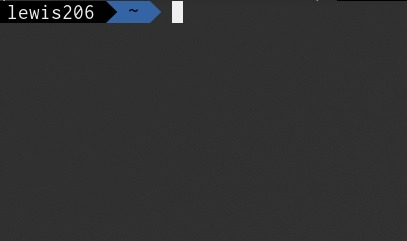
\includegraphics[width=0.7\textwidth]{images/zsh_shell.jpg}
      \caption*{zsh-Shell mit oh-my-zsh agnoster Theme}
      \end{figure}
      \begin{figure}
        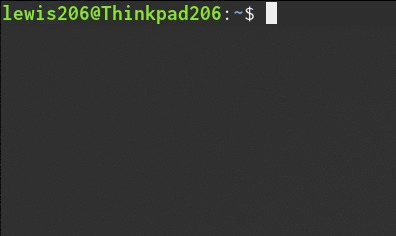
\includegraphics[width=0.7\textwidth]{images/bash_shell.jpg}
      \caption*{bash-Shell}
      \end{figure}
    \end{column}
  \end{columns}
  
\end{frame}


\begin{frame}{Dateisystem}
  \begin{columns}[onlytextwidth]
    \begin{column}{0.475\textwidth}
      \begin{itemize}
        \item bildet \emph{einen} Baum
          \begin{itemize}
            \item beginnt bei \texttt{/} (root)
            \item \texttt{/} trennt Teile eines Pfads
            \item auf Groß-/Kleinschreibung achten!
          \end{itemize}
        \item es gibt ein aktuelles Verzeichnis
        \item relativer Pfad: vom aktuellen Verzeichnis aus (Kein führender \alert{/})
        \item absoluter Pfad: von \alert{/} aus
        \item spezielle Verzeichnisse:
          \begin{description}[\texttt{..}]
            \item[\texttt{.}] das aktuelle Verzeichnis
            \item[\texttt{..}] das Oberverzeichnis
            \item[\texttt{\textasciitilde}] das Home-Verzeichnis
          \end{description}
      \end{itemize}
    \end{column}
  \end{columns}
  \begin{tikzpicture}[
      tree layout,
      font=\ttfamily\bfseries\Large,
      shift={(12, 5)},
      remember picture,
      overlay,
    ]
    \graph[grow down] {
      "/" -> {
        "home/" -> {
          "mnoethe/" -> {
            "Documents/" -> "Example.tex",
            ".zshrc",
          },
          "jluckey/",
        }, 
        "etc/",
        "data/"
      }
    };
  \end{tikzpicture}
\end{frame}

\begin{frame}{\texttt{ls}, \texttt{cd}, \texttt{pwd}}
  \begin{tabu}{>{\ttfamily}l X[,L]}
    ls [\textit{directory}] & \enquote{list}: zeigt den Inhalt eines Verzeichnisses an \\
    ls -l                   & \enquote{long}: zeigt mehr Informationen über Dateien und Verzeichnisse \\
    ls -a                   & \enquote{all}: zeigt auch versteckte Dateien (fangen mit \texttt{.} an) \\
    cd \textit{directory} & \enquote{change directory}: wechselt in das angegebene Verzeichnis\\
    cd - & Wechselt ins vorherige Verzeichnis zurück \\
    pwd                   & \enquote{print working directory}: zeigt das aktuelle Verzeichnis \\
  \end{tabu}
\end{frame}

\begin{frame}{\texttt{mkdir}, \texttt{touch}}
  \begin{tabu}{>{\ttfamily}l X[,L]}
    mkdir \textit{directory}    & \enquote{make directory}: erstellt ein neues Verzeichnis \\
    mkdir -p \textit{directory} & \enquote{parent}: erstellt auch alle notwendigen Oberverzeichnisse \\
    touch \textit{file}         & erstellt eine leere Datei, falls sie noch nicht existiert \\
                                & ändert Bearbeitungsdatum auf \enquote{jetzt}
  \end{tabu}
\end{frame}

\begin{frame}{\texttt{cp}, \texttt{mv}, \texttt{rm}, \texttt{rmdir}}
  \begin{tabu}{>{\ttfamily}l X[,L]}
    cp \textit{source} \textit{destination}    & \enquote{copy}: kopiert eine Datei \\
    cp -r \textit{source} \textit{destination} & \enquote{recursive}: kopiert ein Verzeichnis rekursiv \\
    mv \textit{source} \textit{desination}     & \enquote{move}: verschiebt eine Datei (Umbenennung) \\
    rm \textit{file}                           & \enquote{remove}: löscht eine Datei (Es gibt keinen Papierkorb!) \\
    rm -r \textit{directory}                   & \enquote{recursive}: löscht ein Verzeichnis rekursiv \\
    rmdir \textit{directory}                   & \enquote{remove directory}: löscht ein \emph{leeres} Verzeichnis
  \end{tabu}
\end{frame}


\begin{frame}[fragile]{\texttt{man}, \texttt{cat}, \texttt{less}, \texttt{grep}, \texttt{echo}}
  \begin{tabu}{>{\ttfamily}l X[,L]}
    man \textit{topic}    & \enquote{manual}: zeigt die Hilfe für ein Programm \\
    cat \textit{file}                           & \enquote{concatenate}: gibt Inhalt einer (oder mehr) Datei(en) aus \\
    less \textit{file}                          & (besser als \texttt{more}): wie \texttt{cat}, aber navigabel \\
    grep \textit{pattern} \textit{file}         & \texttt{g/re/p}: sucht in einer Datei nach einem Muster \\
    grep -i \textit{pattern} \textit{file}      & \enquote{case insensitive} \\
    grep -r \textit{pattern} \textit{directory} & \enquote{recursive}: suche rekursiv in allen Dateien \\
    echo \textit{message}                       & gibt einen Text aus
  \end{tabu}

  Beispiel: Finde jedes Paket, dass wir in unseren Python-Skripten importieren:
  
  \begin{lstlisting}[language=bash]
    $ grep -R --include='*.py' import
    v52_leitungen/scripts/plot_lcrg.py:import matplotlib.pyplot as plt
    v52_leitungen/scripts/plot_lcrg.py:import numpy as np
  \end{lstlisting}

\end{frame}

\begin{frame}[fragile]{\texttt{find}}
  Sehr mächtiges Werkzeug, um Dateien und Ordner zu finden, und Befehle auszuführen.

  \begin{tabu}{>{\ttfamily}l X[,L]}
    find . & Rekursiv alle Dateien und Ordner im aktuellen Verzeichnis listen \\
    find . -type f & Nur Dateien anzeigen \\
    find . -name '*.py' & Alle Dateien, die mit \texttt{.py} enden \\
    find . -exec <befehl> \textbackslash{}; & Befehl für jede gefundene Datei ausführen, \texttt{\{\}} wird durch den Dateinamen ersetzt \\
  \end{tabu}
\end{frame}

\begin{frame}{Ein- und Ausgabe}
  \begin{tabu}{>{\ttfamily}l X[,L]}
    \textit{command} > \textit{file}      & überschreibt Datei mit Ausgabe \\
    \textit{command} >> \textit{file}     & fügt Ausgabe einer Datei hinzu \\
    \textit{command} < \textit{file}      & Datei als Eingabe \\
    \textit{command1} | \textit{command2} & Ausgabe als Eingabe (Pipe)
  \end{tabu}
\end{frame}

\begin{frame}{Globbing}
  \begin{tabu}{>{\ttfamily}l X[,L]}
    *                         & wird ersetzt durch alle passenden Dateien \\
    \{\textit{a},\textit{b}\} & bildet alle Kombinationen
  \end{tabu}

  \vspace{2cm}
  Beispiele:\\[10pt]
  \begin{tabu}{>{\ttfamily}l c >{\ttfamily}l}
    *.log           & → & foo.log bar.log \\
    foo.\{tex,pdf\} & → & foo.tex foo.pdf
  \end{tabu}
\end{frame}

\begin{frame}[fragile]{User, Gruppen, Rechte}
  \begin{itemize}
    \item Jede Datei hat einen Besitzer und eine Gruppe
    \item Lese-, Schreib- und Ausführungsrechte können einzeln vergeben werden
    \begin{verbatim}
-rwxr-xr-x  1 maxnoe maxnoe  177 15. Sep 13:37 toggle-touchpad.sh
-rw-r--r--  1 maxnoe maxnoe  98K 29. Aug 15:52 trigger_arduino.jpg
-rw-r--r--  1 maxnoe maxnoe  410 13. Jul 10:37 trigger.py
drwxr-xr-x 20 maxnoe maxnoe 4.0K 29. Sep 11:19 Uni
 \_/\_/\_/
  U  G  O
  s  r  t
  e  o  h
  r  u  e
     p  r
    \end{verbatim}
    \item \texttt{r}: read, \texttt{w}: write, \texttt{x}: execute 
    \item \texttt{u}: user, \texttt{g}: group, \texttt{o}: other, \texttt{a}: all 
    \item \texttt{d}: Ist Verzeichnis
  \end{itemize}
  
\end{frame}

%% chmod frame
\begin{frame}{\texttt{chmod}, \texttt{sudo}}
  \begin{tabu}{>{\ttfamily}l X[,L]}
    chmod \textit{[options] mode file1 ...}    & \enquote{change mode}: Verändert die klassischen Unix-Dateirechte  \\
    chmod a+x beispiel.txt    & Beispiel: Fügt bei allen das Recht auf Ausführung hinzu \\
    sudo \textit{command} & \enquote{superuser do}: führt einen Befehl als \enquote{root}-User aus \alert{Achtung}: Mit Vorsicht verwenden!\\
  \end{tabu}
\end{frame}

\begin{frame}{Shell-Skripte}
  \begin{itemize}
    \item Datei enthält Befehle
    \item Selbe Syntax wie Kommandozeile
    \item Endung: keine oder \texttt{.sh}
    \item Ausführung:
      \begin{itemize}
        \item \texttt{bash \textit{skript}}
        \item \texttt{./\textit{skript}} (mit Shebang)
      \end{itemize}
    \item Shebang: erste Zeile enthält Pfad des Interpreters (muss absolut sein)
      \begin{itemize}
        \item \texttt{\#!/bin/bash}
      \end{itemize}
  \end{itemize}
\end{frame}

\begin{frame}{Config-Files}
  \begin{itemize}
    \item Einstellungen für viele Programme werden in Textdateien gespeichert
    \item Üblicherweise versteckte Dateien im \texttt{HOME}-Verzeichnis
    \item Einstellungen für die Konsole an sich: \texttt{.bashrc}, \texttt{.zshrc}, etc.
    \item Bash-Befehle die beim Start jeder Konsole ausgeführt werden
    \item Umgebungsvariablen setzen
    \item Sehr nützlich: \texttt{alias}, definiert Alternativform für Befehle \\
      \texttt{alias ll='ls -lh'} \\
      \texttt{alias gits='git status -s'} \\
      \texttt{alias ..='cd ..'}
    \item Müssen nach Änderungen neugeladen werden:\\
      \texttt{source \textasciitilde/.bashrc}
  \end{itemize}
\end{frame}

\begin{frame}{Umgebungsvariablen}
  \begin{itemize}
    \item steuern viele Einstellungen und Programme
    \item Ausgabe mit \texttt{echo \$NAME}
    \item wichtiges Beispiel: \texttt{PATH} (auch unter Windows):
      \begin{itemize}
        \item enthält alle Pfade, in denen nach Programmen gesucht werden soll
        \item wird von vorne nach hinten gelesen
        \item erster Treffer wird genommen
        \item \texttt{which \textit{program}} zeigt den Pfad eines Programms
        \item Shebang, das den ersten Treffer im \texttt{PATH} nutzt, statt festem Pfad: \texttt{\#!/usr/bin/env python}
      \end{itemize}
    \item Änderung über \texttt{export}:\\
      \texttt{export PATH=\$HOME/.local/texlive/2021/bin/x86\_64-linux:\$PATH}
  \end{itemize} 
\end{frame}

